\subsubsection{Testfall: Freier Fluss}
Anhand dieses Testszenarios soll überprüft werden, ob sich die Personen auf freier Strecke mit ihrer individuellen Wunschgeschwindigkeit fortbewegen. Abbildung \ref{fig:freeflowVGLmap} zeigt das verwendete Feld. Die Simulation wurde auf Basis des Euklid Algorithmus durchgeführt. Die Entfernung vom Ziel zur Person beträgt $25,31\ m$. Die Simulationszeit beträgt $21,90\ s$s. Daraus ergibt sich eine mittlere Geschwindigkeit von $1,16 m/s$. Die Auswertung der tatsächlich gelaufenen Geschwindigkeit ($velocity.csv$) ergibt, dass die Person zu jedem Messzeitpunkt mit ihrer individuellen Wunschgeschwindigkeit von $1.21 m/s$ läuft. \\
Es ist festzustellen, dass die Person nicht den optimalen Weg läuft. In der Abbildung ist der optimale Weg $blau$ und der tatsächlich gelaufene Weg $violett$ hervorgehoben. Diese Abweichung ist darauf zurückzuführen, dass sich die Person nur in 8 Richtungen (Moore-Umgebung) bewegen kann. Für diesen Test wurde explizit eine Karte gewählt, in der die Person nicht ausschließlich diagonal ins Ziel gelangen kann. \\
Daraus ergeben sich folgende Problematiken: Die Person ist nicht in der Lage den optimalen Weg zu wählen. Das entspricht nicht der Realität. Dieser Umweg muss bei der Bewertung der Simulationsergebnisse beachtet werden. Durch die lediglich 8 möglichen Bewegungsrichtungen ergeben sich verschiedene Kombinationen von Pfaden mit gleicher Strecke zum Ziel. In diesem Fall ist die Person zunächst diagonal gelaufen und zum Schluss geradeaus. Denkbar wäre auch ein Pfad, bei dem dies umgekehrt wäre. Eine dritte Option wäre beispielsweise, dass die Person abwechselnd geradeaus und diagonal läuft.

\begin{figure}[ht]
	\centering
	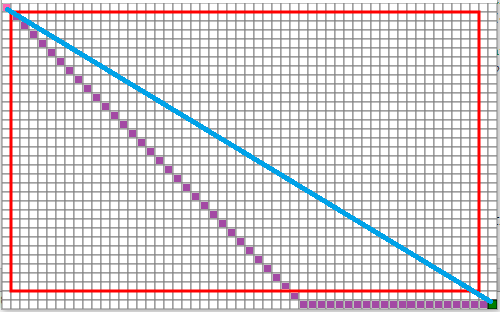
\includegraphics[width=\textwidth]{abbildungen/freeflowVGL.png}
	\caption{Feld des Testfalls, Optimaler Weg (blau) und gewählter Weg (violett)}
	\label{fig:freeflowVGLmap}
\end{figure}